\chapter{Марий или Сулла - кто круче?}

Граждане интересуются, кто самый крутой римлянин первого этапа римских гражданских войн, Гай Марий или Люций Корнелий Сулла. Сравнение исторических персонажей всегда натягивание совы на глобус, дело достаточно бессмысленное, но увлекательное. Поэтому почему бы и не сравнить.


Для начала оценим кто кого, нефигурально выражаясь, прикопал. Тут нам мешает разница в возрасте - 20 лет. Когда Марий был в возрасте Суллы (под полтинник), он запиздошил своего непосредственного начальнике, перехватил контроль над армией через политические рычаги и выиграй ей войну в Нумидии, а потом вернулся в Италию и неиллюзорно спас Рим от тотального кимврского пиздеца, за что ему респектосики. Ну и бессрочные консульства, крутые реформы, Марий был просто рок-звезда, и даже Илон Маск от такого масштаба личности и масштаба свершений охуел бы. Но мы проматываем 20 лет, и вуаля, Мария спустили с небес на землю, и старикан уже был в своем закате, а против него выходит он же, но на двадцать лет моложе, и гнет его в бараний рог. Крч, в этом плане, "кто круче", сравнивать их тяжело, разные поколения совсем. Но Сулла моложе, он на пике формы, и именно он накидал пиздюлей марианцам а не наоборот, поэтому отдам первый голос за Суллу. Дети должны выебать своих отцов когда те постареют, ослабнут и потеряют хватку, иначе они хуевые дети и вырожденцы. И Сулла доказал что достоин своего поколения.


По эпичности побед, если обьективно сравнивать, то они почти равны. Да, Третья Митридатовая, вся хуйня, а потом ещё Гражданская. Но инструменты для опиздюдивания внешних и внутренних врагов дал Марий, продвигал Суллу на ранних этапах тоже Марий, плюс сами по себе гражданские войны штука аморальная и триумфов за них не положено. А карта Митридата бьется Кимврской войной, куда более страшной для Республики, чем понтийский сатрап, насколько бы он там не был крут и могущественен. Кимвры били в центр Италии, и у них получалось, что самое страшное. Даже по масштабам изменений видно насколько Кимврская война важна там мало того что военная реформа и обострение конфликта популяров с оптиматами, а ровно через десять лет ебанула Союзническая война, прямое следствие того, что италики во главе с Марием затащили нашествие кимвров. В общем, я бы их поставил примерно на один уровень, Митридатову и Кимврскую, а гражданскую вообще оставил за скобками. Но у Мария есть в активе война с Югуртой, его первая успешная кампания, причем длящаяся уже пару лет к тому моменту, и Рим в ней просирал. А Марий вытянул. И это перевешивает чашу весов, поэтому за военную доблесть я отдаю балл Марию.


Далее, политичая карьера. Вот тут кто всё проебал? Марий всё проебал. Да, у него был золотой век, четыре консульства подряд и карт-бланш на всё. Но он был недолог, а потом его слили, и даже Сатурнин не помог. Да и дальнейшая его политическая карьера это сплошной позор. Тогда как Сулла сотворил куда больше, причем лично, в отличии от Мария. Именно его воля, ум, и его понимание как надо обустроить Республику позволили ему вытащить внешнюю войну, а потом развернуться и затащить войну внутренню. А уж проскрипции это вообще шикарно. Собственно, самые важные сулланские новаторства это первое в истории взятие Рима собственными войсками (он брал Рим дважды, первый раз почти без боя, а второй достаточно кроваво), тоесть использование армии для решения политических вопросов. И это проскрипции, тоесть избирательная резня своих политических оппонентов. Вот это, блядь, новаторство так новаторство, после него город брали раз десять, а патрициев резали постоянно. Да, Октавиан повторил проскрипционные списки "на бисс", но по тихой сапе тупо убивать оппонентов при первой возможности начали именно после Суллы, до этого соблюдался политес (про Гракхов не вспоминаем, они поэтому и так значимы, так как исключение и "так не принято" было). В общем, тут я однозначно отдам балл Сулле, Марию до него далеко. "Последний раз, когда войска Суллы брали Город - стены можно было красить кровью", хехе.


А вот живучесть идей, это другое дело. При жизни Сулла добился всего чего хотел, плыл против течения в серной кислоте и приплыл куда требовалось, а потом убил там всех кого требовалось и наступил мир. А потом он умер, и уже через десятиление всё пошло по пизде и его же собственные Красс с Помпеем откатили взад практически всё его политическое наследие. А вот Марий, хоть при жизни и проебал, но в итоге Цезарь у нас марианец, тоесть популяр, и Октавиан тоже. Да и Антоний тоже, и Лепид. Собственно, в финал гражданской войны вышли одни марианцы, и рубились кто из них более популяр, а сулланцы всё проебали, "последний катончик остыл, последний сенатик устал". Идеи Мария были более адекватны будущему, более живучие и в итоге они победили, а сулланская модель показала свою ущербность вскоре после смерти своего создателя. Так что тут Марий ван лав.


Вот такие пироги. Со счетом 2:2 я признаю это исторический версус-батол закончившимся ничьей. Dixi.



\begin{figure}[h!tb] 
	\centering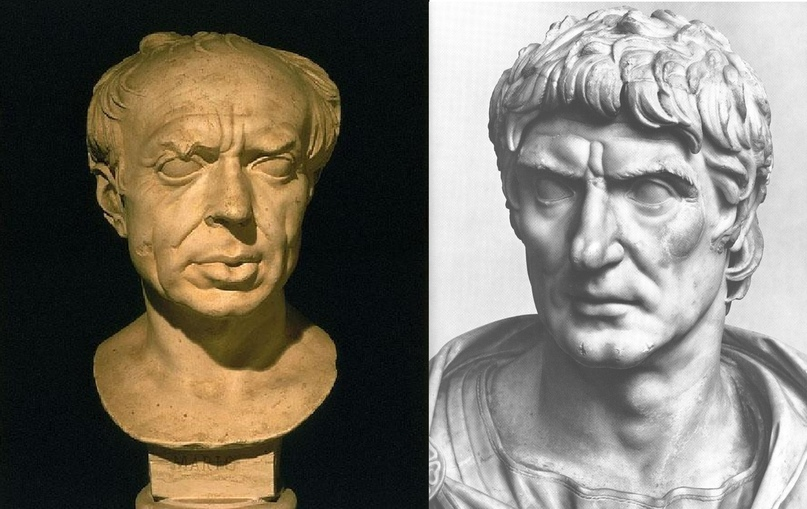
\includegraphics[scale=0.6]{SullaMariy/1595005110125645377.png}
	%	\label{fig:scipion} % Unique label used for referencing the figure in-text\end{document}
	%	%\addcontentsline{toc}{figure}{Figure \ref{fig:placeholder}} % Uncomment to add the figure to the table of contents%----------------------------------------------------------------------------------------
	\caption{На картинке  слева Марий а справа Сулла.}%	CHAPTER 2
\end{figure}